\documentclass[11pt]{scrartcl}
\usepackage[T1]{fontenc}
\usepackage[a4paper, left=3cm, right=2cm, top=2cm, bottom=2cm]{geometry}
\usepackage[activate]{pdfcprot}
\usepackage[ngerman]{babel}
\usepackage[parfill]{parskip}
\usepackage[utf8]{inputenc}
\usepackage{kurier}
\usepackage{amsmath}
\usepackage{amssymb}
\usepackage{xcolor}
\usepackage{epstopdf}
\usepackage{txfonts}
\usepackage{fancyhdr}
\usepackage{graphicx}
\usepackage{prettyref}
\usepackage{hyperref}
\usepackage{eurosym}
\usepackage{setspace}
\usepackage{units}
\usepackage{eso-pic,graphicx}
\usepackage{icomma}

\definecolor{darkblue}{rgb}{0,0,.5}
\hypersetup{pdftex=true, colorlinks=true, breaklinks=false, linkcolor=black, menucolor=black, pagecolor=black, urlcolor=darkblue}



\setlength{\columnsep}{2cm}


\newcommand{\arcsinh}{\mathrm{arcsinh}}
\newcommand{\asinh}{\mathrm{arcsinh}}
\newcommand{\ergebnis}{\textcolor{red}{\mathrm{Ergebnis}}}
\newcommand{\fehlt}{\textcolor{red}{Hier fehlen noch Inhalte.}}
\newcommand{\betanotice}{\textcolor{red}{Diese Aufgaben sind noch nicht in der Übung kontrolliert worden. Es sind lediglich meine Überlegungen und Lösungsansätze zu den Aufgaben. Es können Fehler enthalten sein!!! Das Dokument wird fortwährend aktualisiert und erst wenn das \textcolor{black}{beta} aus dem Dateinamen verschwindet ist es endgültig.}}
\newcommand{\half}{\frac{1}{2}}
\renewcommand{\d}{\, \mathrm d}
\newcommand{\punkte}{\textcolor{white}{xxxxx}}
\newcommand{\p}{\, \partial}
\newcommand{\dd}[1]{\item[#1] \hfill \\}

\renewcommand{\familydefault}{\sfdefault}



\newcommand{\themodul}{Probeklausuren 10+11}
\newcommand{\thetutor}{bei Prof. Schöning}

\pagestyle{fancy}
\fancyhead[L]{\footnotesize{C. Hansen}}
\chead{\thepage}
\rhead{}
\lfoot{}
\cfoot{}
\rfoot{}

\title{\themodul{}}
\publishers{\thetutor}


\author{Christoph Hansen \\ {\small \href{mailto:chris@university-material.de}{chris@university-material.de}} }

\date{}

\usepackage{paralist}
\begin{document}

\maketitle

Dieser Text ist unter der
\href{http://creativecommons.org/licenses/by-nc/4.0/}{Creative Commons CC BY-NC 4.0}
Lizenz veröffentlicht.

\textcolor{red}{%
    Ich erhebe keinen Anspruch auf Vollständigkeit oder Richtigkeit. Falls ihr
    Fehler findet oder etwas fehlt, dann meldet euch bitte über den
    Emailkontakt.
}


\tableofcontents

\newpage


\section{Klausur 10}

\subsection{Aufgabe 1}

Bei dieser Aufgabe bin ich mir nicht sicher, ob die jeweiligen Lösungen korrekt sind. Wenn jemand begründet eine bessere hat, dann soll er sich melden.

\hfill\\

\begin{center}
\begin{tabular}{c|c|c|c|c|c|c|c|c|c}
a) & b) & c) & d) & e) & f) & g) & h) & i) & j) \\ 
\hline 
F & F & R & F & F & R & F & R & R & F \\ 
\end{tabular} 

\end{center}


\subsection{Aufgabe 2}

\subsubsection*{a)}

mechanisch, thermisch, optisch, akustisch

\subsubsection*{b)}

\begin{figure}[h]
\centering
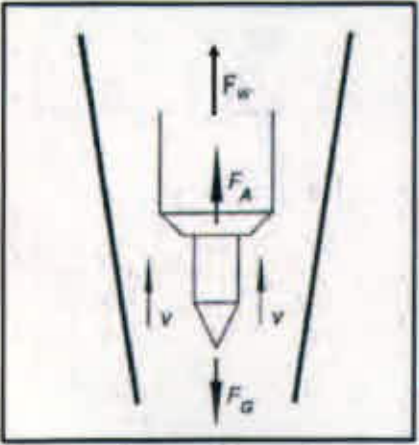
\includegraphics[scale=0.6]{A2b.png}
\caption{$F_A$: Auftriebskraft, $F_W$: Widerstandskraft, $F_G$: Gewichtskraft}
\end{figure}

Der zu messende Luftstrom wird von unten in die Apparatur eingeleitet und drückt den Schwebekörper nach oben. Nachdem sich der Schwebekörper auf eine konstante Höhe eingependelt hat, kann man die Durchflussmenge anhand der Höhe bestimmen.


\end{document}
